\documentclass[a4paper,11pt]{article}

\usepackage[T1]{fontenc}
\usepackage[utf8]{inputenc}
\usepackage{graphicx}
\usepackage{xcolor}

\renewcommand\familydefault{\sfdefault}
\usepackage{tgheros}

\usepackage{amsmath,amssymb,amsthm,textcomp}
\usepackage{enumerate}
\usepackage{multicol}
\usepackage{tikz}

\usepackage{geometry}
\geometry{left=25mm,right=25mm,%
bindingoffset=0mm, top=20mm,bottom=20mm}

\usepackage[export]{adjustbox}
\usepackage{subcaption}
\usepackage{float}


\linespread{1.3}

\newcommand{\linia}{\rule{\linewidth}{0.5pt}}

% custom theorems if needed
\newtheoremstyle{mytheor}
    {1ex}{1ex}{\normalfont}{0pt}{\scshape}{.}{1ex}
    {{\thmname{#1 }}{\thmnumber{#2}}{\thmnote{ (#3)}}}

\theoremstyle{mytheor}
\newtheorem{defi}{Definition}

% my own titles
\makeatletter
\renewcommand{\maketitle}{
\begin{center}
\vspace{2ex}
{\huge \textsc{\@title}}
\vspace{1ex}
\\
\linia\\
\@author \hfill \@date
\vspace{4ex}
\end{center}
}
\makeatother
%%%

% custom footers and headers
\usepackage{fancyhdr}
\pagestyle{fancy}
\lhead{}
\chead{}
\rhead{}
\lfoot{Analiza Algorytmów, lab 3}
\cfoot{}
\rfoot{Page \thepage}
\renewcommand{\headrulewidth}{0pt}
\renewcommand{\footrulewidth}{0pt}
%

\graphicspath{ {../data/png/} }

%%%----------%%%----------%%%----------%%%----------%%%

\begin{document}

\title{Analiza Algorytmów, lab 3}

\author{Adrian Mucha, Politechnika Wrocławska, WPPT}

\date{12/05/2020}

\maketitle

\section*{Zad 11}
Niech $0 < q < \frac{1}{2}$ oznacza prawdopodobieństwo wydobycia kolejnego bloku przez adwersarza odpowiadające części mocy obliczeniowej będącej w jego posiadaniu.

Niech $n$ oznacza liczbę potwierdzeń (nadbudowanych bloków) potrzebnych by uznać transakcję za potwierdzoną.

Niech $P(n, q)$ oznacza prawdopodobieństwo, że adwersarz o mocy $q$ będzie dysponował łańcuchem bloków równym lub
dłuższym niż ten budowany przez uczciwych użytkowników w momencie, gdy nadbudowali oni blok zawierający rozważaną transakcję $n$ blokami lub kiedykolwiek później.

\subsection*{Opis symulacji ataku \emph{,,double spending"} (metoda Monte Carlo)}
Pojedyncze doświadczenie polega na pobraniu $10000$ próbek wydarzeń
$$P(n, q) = \emph{adwersarz wygrywa atak ,,double spending"},$$
oraz ich uśrednieniu. Doświadczenie rozpoczyna się postawieniem zadania wykopania $n$ bloków \emph{dobrym użytkownikom}, którzy wykonają tę pracę w czasie $t\in(0, \infty)$. W każdej jednostce czasu \emph{użytkownik} ma $p = 1 - q$ szans na wykopanie $1$ bloku. \emph{Adwersarz} w tym samym czasie $t$, kopie $k$ bloków (ma tyle samo prób co \emph{użytkownik}). Jeżeli $k \geq n$ to zdarzenie $P(n, q)$ uznajemy za \emph{sukces}.

\subsection*{Nakamoto vs. Grunspan vs. otrzymane wyniki}
\begin{figure}[H]
    \begin{subfigure}{0.5\textwidth}
        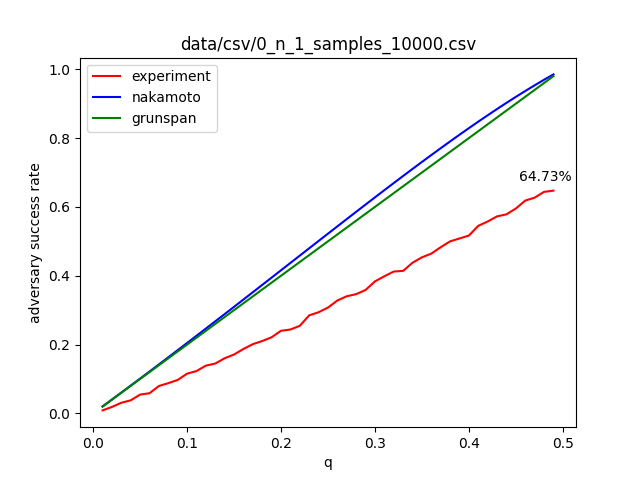
\includegraphics[width=1.0\linewidth]{0_n_1_samples_10000.png}
        \caption{$n = 1$}
        \label{fig:subim1}
    \end{subfigure}
    \begin{subfigure}{0.5\textwidth}
        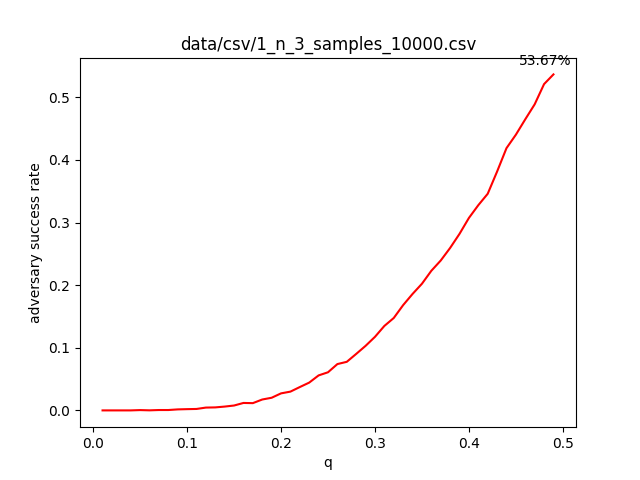
\includegraphics[width=1.0\linewidth]{1_n_3_samples_10000.png}
        \caption{$n = 3$}
        \label{fig:subim2}
    \end{subfigure}

    \begin{subfigure}{0.5\textwidth}
        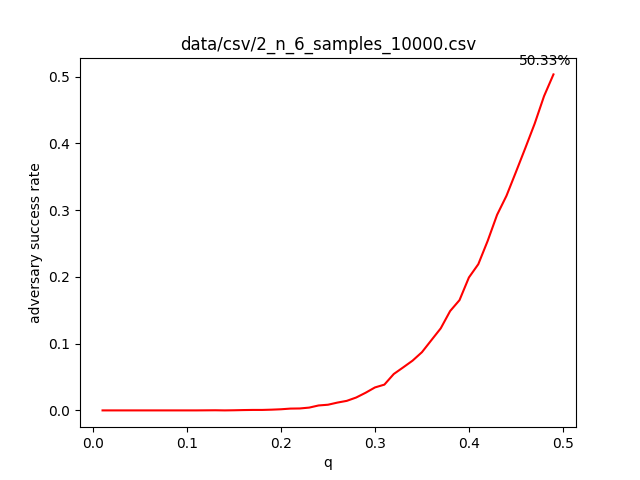
\includegraphics[width=1.0\linewidth]{2_n_6_samples_10000.png}
        \caption{$n = 6$}
        \label{fig:subim3}
    \end{subfigure}
    \begin{subfigure}{0.5\textwidth}
        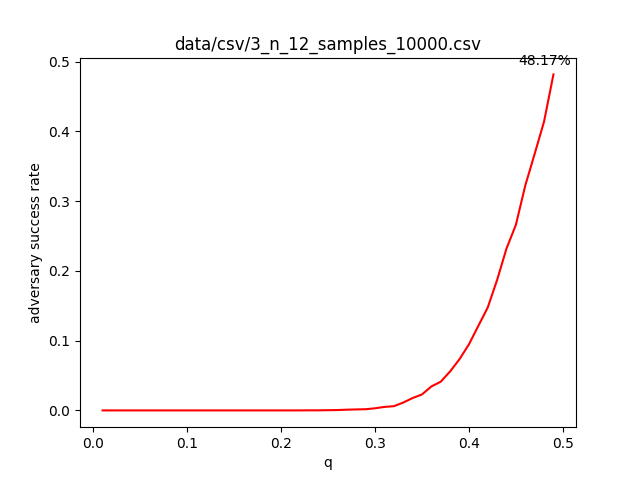
\includegraphics[width=1.0\linewidth]{3_n_12_samples_10000.png}
        \caption{$n = 12$}
        \label{fig:subim4}
    \end{subfigure}

    \begin{subfigure}{0.5\textwidth}
        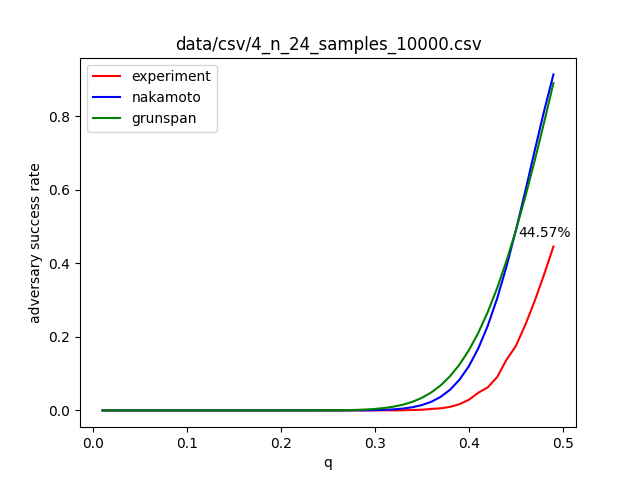
\includegraphics[width=1.0\linewidth]{4_n_24_samples_10000.png}
        \caption{$n = 24$}
        \label{fig:subim5}
    \end{subfigure}
    \begin{subfigure}{0.5\textwidth}
        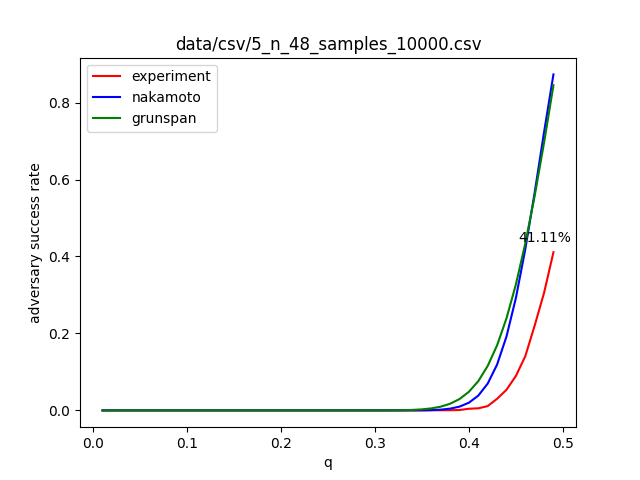
\includegraphics[width=1.0\linewidth]{5_n_48_samples_10000.png}
        \caption{$n = 48$}
        \label{fig:subim6}
    \end{subfigure}

    \caption{\footnotesize Wykresy przedstawiają prawdopodobieństwo sukcesu adwersarza w zależności od parametru $q$. Kolor {\color{red} czerwony} prezentuje otrzymane wyniki gdy uruchomiono symulację $10000$ razy dla każdego $0 < q < 0.5$ i uśredniono. Kolejno kolorem {\color{green} zielonym} oraz {\color{blue} niebieskim} oznaczono formuły autorów Grunspan'a oraz Nakamoto. Jak można zauważyć, formuły narzucone przez wcześniej wspomnianych autorów są bardziej restrykcyjne. W punkcie gdy atakujący posiada niemal połowę dostępnej mocy obliczeniowej, autorzy twierdzą, że prawdopodobieństwo wygrania przez adwersarza jest prawie pewne, natomiast w danych z eksperymentu wynika iż zbliża się on jedynie do $\frac{1}{2}$ szansy na powodzenie ataku "double spending".}
    \label{fig:data1}
\end{figure}

\subsection*{Jak dobrać $n$ przy dopuszczalnym prawdopodobieństwie sukcesu adwersarza $P(n, q) \leq \alpha$ w zależności od $q$}
\begin{figure}[H]
    \begin{subfigure}{0.5\textwidth}
        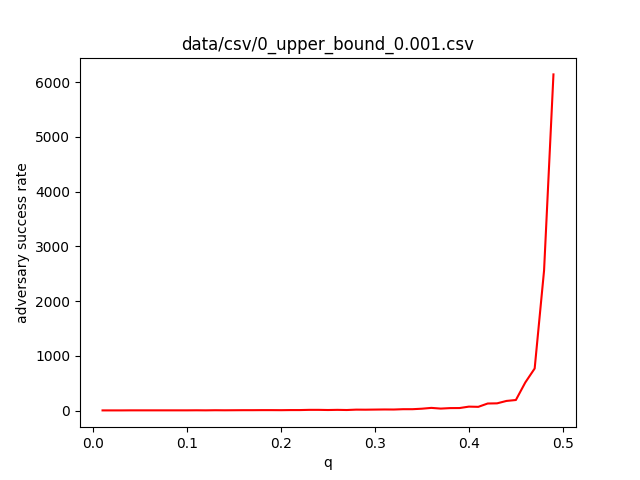
\includegraphics[width=1.0\linewidth]{0_upper_bound_0.001.png}
        \caption{$P(n, q) = 0,1\%$}
        \label{fig:subim1}
    \end{subfigure}
    \begin{subfigure}{0.5\textwidth}
        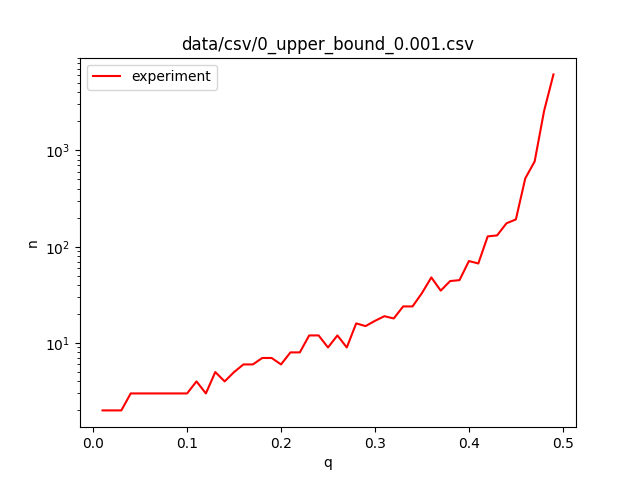
\includegraphics[width=1.0\linewidth]{0_upper_bound_log_0.001.png}
        \caption{$P(n, q) = 0,1\%$ (skala logarytmiczna)}
        \label{fig:subim1}
    \end{subfigure}

    \begin{subfigure}{0.5\textwidth}
        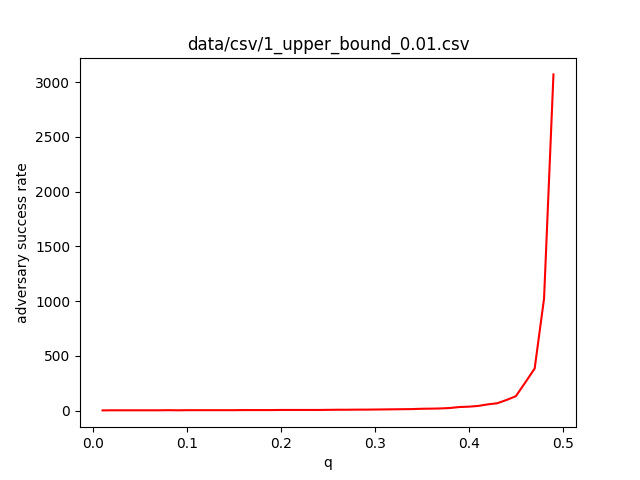
\includegraphics[width=1.0\linewidth]{1_upper_bound_0.01.png}
        \caption{$P(n, q) = 1\%$}
        \label{fig:subim1}
    \end{subfigure}
    \begin{subfigure}{0.5\textwidth}
        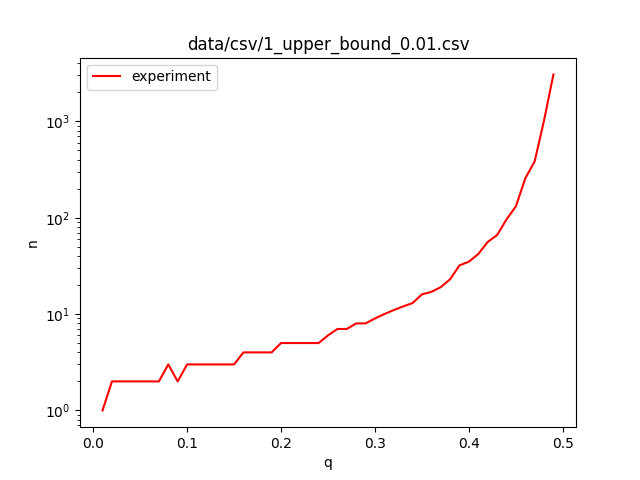
\includegraphics[width=1.0\linewidth]{1_upper_bound_log_0.01.png}
        \caption{$P(n, q) = 1\%$ (skala logarytmiczna)}
        \label{fig:subim1}
    \end{subfigure}

    \begin{subfigure}{0.5\textwidth}
        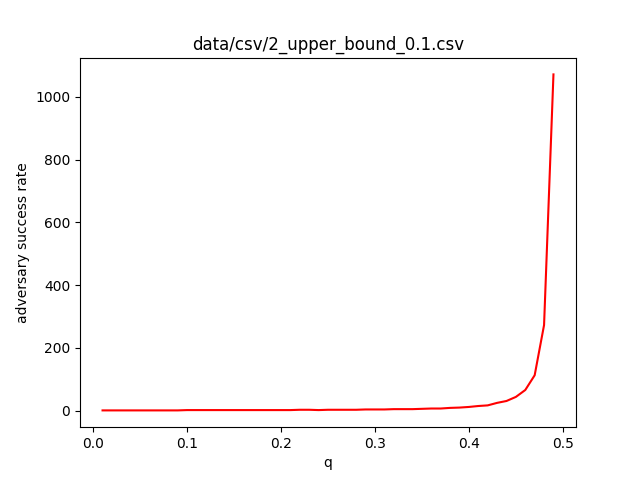
\includegraphics[width=1.0\linewidth]{2_upper_bound_0.1.png}
        \caption{$P(n, q) = 10\%$}
        \label{fig:subim1}
    \end{subfigure}
    \begin{subfigure}{0.5\textwidth}
        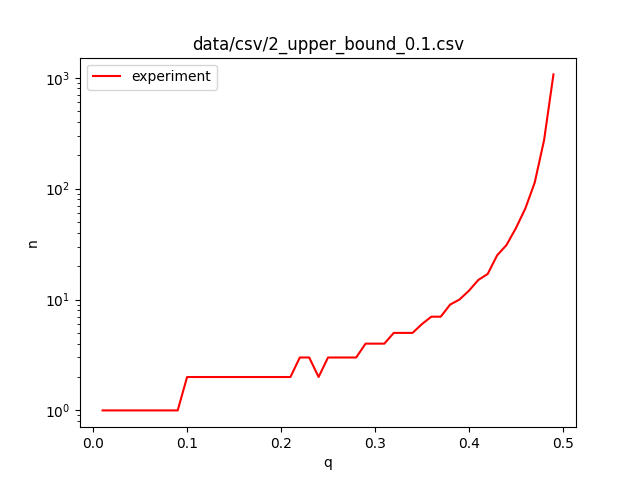
\includegraphics[width=1.0\linewidth]{2_upper_bound_log_0.1.png}
        \caption{$P(n, q) = 10\%$ (skala logarytmiczna)}
        \label{fig:subim1}
    \end{subfigure}

    \caption{Można zauważyć, że gdy adwersarz dysponuje mocą bliską $\frac{1}{2}$ całej mocy obliczeniowej to wartość $n$ drastycznie wzrasta by móc spełnić warunek dopuszczalnego prawdopodobieństwa adwersarza.}
    \label{fig:data2}
\end{figure}

\end{document}